\documentclass[11pt,a4paper]{article}
\usepackage[T1]{fontenc}
\usepackage{microtype}
\usepackage[margin=29mm,headheight=14pt]{geometry}
\usepackage{amsmath,amsthm,amssymb,mathtools}
\usepackage{newtxtext,newtxmath}
\usepackage{tikz}
\usetikzlibrary{calc,arrows.meta,patterns}
\usepackage{caption,booktabs}
\usepackage[unicode,hidelinks]{hyperref}
\usepackage{fancyhdr}
\pagestyle{fancy}\fancyhf{}\fancyhead[L]{\footnotesize \textit{Sombor products on trees}}\fancyhead[R]{\footnotesize T. Newton}\fancyfoot[C]{\thepage}\renewcommand{\headrulewidth}{0.25pt}
\numberwithin{equation}{section}
\newtheorem{theorem}{Theorem}[section]
\newtheorem{lemma}[theorem]{Lemma}
\newtheorem{proposition}[theorem]{Proposition}
\newcommand{\somb}{\operatorname{SO}}
\newcommand{\msomb}{\operatorname{{}^m SO}}
\newcommand{\prodso}{\operatorname{\pi SO}}
\newcommand{\Es}{E_{d,k}}
\newcommand{\dd}{\mathrm{d}}
\newcommand{\floor}[1]{\left\lfloor #1\right\rfloor}
\title{The maximum product of the Sombor and modified Sombor indices of a tree}
\author{Tony Newton}
\date{}
\begin{document}
\maketitle
\vspace{-2.0em}
\begin{abstract}
The Sombor index and its modified counterpart weight each edge of a graph by the Euclidean norm of its endpoint degrees and the reciprocal of that norm. Their product measures the variation of those weights across the graph, and its maximum over trees is not determined by maximizing either factor separately. Gutman, Red\v{z}epovi\'{c}, and Furtula conjectured in 2023 that an $n$-vertex tree maximizing this product is a specific eclipsed sun. We prove their sharp inequality and the uniqueness of the extremizer for every $n\geq5$. The proof first excludes trees without a dominant-degree vertex, then compares the remaining trees directly with eclipsed suns by a nonnegative edge defect, and finally obtains the optimal arm count by signed finite differences. The infinite families are treated analytically; finite exceptional ranges are resolved by exact rational intervals and enumeration of unlabeled trees. The result settles the stated extremal-tree conjectures, not the unrelated questions concerning chemical correlations of the index.
\end{abstract}
\noindent\textbf{Keywords:} Sombor index; modified Sombor index; tree; extremal graph; degree sequence.\par
\noindent\textbf{MSC 2020:} 05C09, 05C35, 05C92.

\section{Introduction and the main result}
For a finite simple graph $G$, denote its vertex and edge sets by $V(G)$ and $E(G)$, and write $d_v$ for the degree of a vertex $v$. The Sombor and modified Sombor indices are
\begin{equation}\label{eq:indices}
\somb(G)=\sum_{uv\in E(G)}\sqrt{d_u^2+d_v^2},\qquad
\msomb(G)=\sum_{uv\in E(G)}\frac1{\sqrt{d_u^2+d_v^2}}.
\end{equation}
Their product $\prodso(G)=\somb(G)\msomb(G)$ was studied by Gutman, Red\v{z}epovi\'{c}, and Furtula~\cite{GRF2023}. The two factors often behave in opposing ways under changes to a graph. If $w_e=\sqrt{d_u^2+d_v^2}$ for $e=uv$ and $m=|E(G)|$, the identity
\begin{equation}\label{eq:dispersion}
\biggl(\sum_e w_e\biggr)\biggl(\sum_e\frac1{w_e}\biggr)
=m^2+\sum_{e<f}\left(\frac{w_e}{w_f}+\frac{w_f}{w_e}-2\right)
\end{equation}
shows why the product is sensitive to unequal edge types. Although the universal lower bound $m^2$ follows from Cauchy--Schwarz, the maximum over trees is a more delicate structural problem.

A tree with one central vertex and arms of lengths one and two is called an \emph{eclipsed sun}. Let $E_{d,k}$ be obtained by subdividing precisely $k$ edges of a $d$-edge star, where $0\le k\le d$. It has $n=d+k+1$ vertices, $k$ arms of length two, and $d-k$ pendent arms of length one; it is the tree denoted $ES(n,k)$ in~\cite{GRF2023}. The three edge types are illustrated in Figure~\ref{fig:sun}. Set
\begin{equation}\label{eq:constants}
a=\sqrt5,\qquad B_d=\sqrt{d^2+4},\qquad C_d=\sqrt{d^2+1}.
\end{equation}
The product for an eclipsed sun is explicit:
\begin{align}
S(E_{d,k})&=dC_d+k(a+B_d-C_d),\label{eq:Ssun}\\
R(E_{d,k})&=\frac{d}{C_d}+k\left(\frac1a+\frac1{B_d}-\frac1{C_d}\right),\label{eq:Rsun}
\end{align}
where for brevity $S=\somb$, $R=\msomb$, and $P=SR=\prodso$.

\begin{figure}[htbp]
\centering
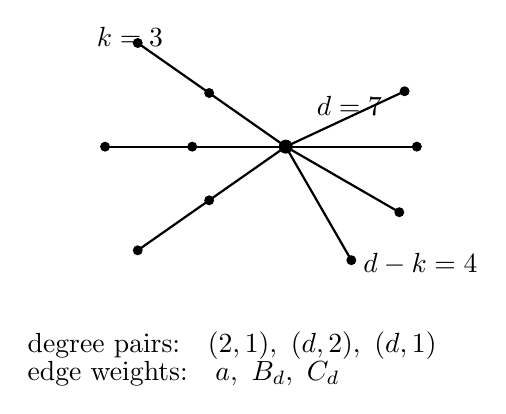
\begin{tikzpicture}[scale=0.9, every node/.style={inner sep=0pt}]
\coordinate (O) at (0,0);
\foreach \ang in {145,180,215} {
  \path (O) ++(\ang:1.32) coordinate (A\ang);
  \path (O) ++(\ang:2.55) coordinate (B\ang);
  \draw[thick] (O)--(A\ang)--(B\ang);
  \fill (A\ang) circle (2.0pt);\fill (B\ang) circle (2.0pt);
}
\foreach \ang in {300,330,0,25} {
  \path (O) ++(\ang:1.85) coordinate (C\ang);
  \draw[thick] (O)--(C\ang);\fill (C\ang) circle (2.0pt);
}
\fill (O) circle (2.8pt);
\node[above right,xshift=11pt,yshift=11pt] at (O) {$d=7$};
\node[above] at (-2.2,1.4) {$k=3$};
\node[below] at (1.9,-1.5) {$d-k=4$};
\node[anchor=west] at (-3.65,-2.8) {$\text{degree pairs:}\quad (2,1),\ (d,2),\ (d,1)$};
\node[anchor=west] at (-3.65,-3.2) {$\text{edge weights:}\quad a,\ B_d,\ C_d$};
\end{tikzpicture}
\caption{The eclipsed sun $E_{7,3}=ES(11,3)$. Its three edge types, with multiplicities $k$, $k$, and $d-k$, give \eqref{eq:Ssun}--\eqref{eq:Rsun}.}
\label{fig:sun}
\end{figure}

The authors of~\cite{GRF2023} found the expected unique maximizer for all trees through order $17$ and formulated their observation as Conjectures 12 and 13. Here is the sharp result.
\begin{theorem}\label{thm:main}
For every integer $n\ge5$, let
\[
k_0=\floor{\frac{n-2}{3}},\qquad d_0=n-k_0-1.
\]
Every tree $T$ on $n$ vertices satisfies
\begin{equation}\label{eq:main}
P(T)\le
\bigl[k_0a+k_0B_{d_0}+(d_0-k_0)C_{d_0}\bigr]
\left[\frac{k_0}{a}+\frac{k_0}{B_{d_0}}+\frac{d_0-k_0}{C_{d_0}}\right].
\end{equation}
Equality holds if and only if $T\cong E_{d_0,k_0}$.
\end{theorem}

The proof has three distinct steps. First, a degree potential excludes $d\le n/2$ for a maximizing tree of order at least $17$. Second, at fixed dominant degree $d>n/2$, a defect estimate proves that replacing a tree by $E_{d,n-1-d}$ cannot decrease its product. Third, a finite-difference argument selects the unique arm count $k_0$. Figure~\ref{fig:degree-region} records the parameter regions involved; it is an aid to reading the proof rather than independent evidence for the inequality.

\begin{figure}[htbp]
\centering
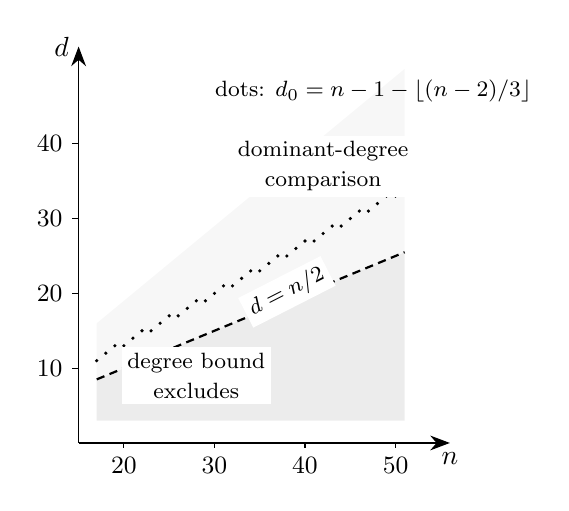
\begin{tikzpicture}[x=0.115cm,y=0.095cm]
 \fill[gray!15] (17,3)--(51,3)--(51,25.5)--(17,8.5)--cycle;
 \fill[gray!6] (17,8.5)--(51,25.5)--(51,50)--(17,16)--cycle;
 \draw[-{Stealth[length=2.5mm]}] (15,0)--(56,0) node[below] {$n$};
 \draw[-{Stealth[length=2.5mm]}] (15,0)--(15,53) node[left] {$d$};
 \foreach \n in {20,30,40,50} {\draw (\n,0)--(\n,-.65) node[below] {\small\n};}
 \foreach \d in {10,20,30,40} {\draw (15,\d)--(14.3,\d) node[left] {\small\d};}
 \draw[densely dashed,thick] (17,8.5)--(51,25.5);
 \node[rotate=27,fill=white,inner sep=2pt] at (38,20.2) {\footnotesize $d=n/2$};
 \foreach \n in {17,...,51} {
   \pgfmathtruncatemacro{\kk}{floor((\n-2)/3)}
   \pgfmathtruncatemacro{\dopt}{\n-\kk-1}
   \fill[black] (\n,\dopt) circle (0.65pt);
 }
 \node[align=center,fill=white,inner sep=2pt] at (28,9) {\footnotesize degree bound\\[-1pt]\footnotesize excludes};
 \node[align=center,fill=white,inner sep=2pt] at (42,37) {\footnotesize dominant-degree\\[-1pt]\footnotesize comparison};
 \node[anchor=west] at (29,47) {\footnotesize dots: $d_0=n-1-\lfloor(n-2)/3\rfloor$};
\end{tikzpicture}
\caption{The two-dimensional $(n,d)$ organization of the proof for $n\ge17$. Below $d=n/2$ the degree-potential bound excludes a maximizer; above the line the defect comparison applies. Dots are the proposed extremal degrees for successive integer orders. The picture displays the exact threshold and integer candidate formula, not sampled values of $P(T)$.}
\label{fig:degree-region}
\end{figure}

\section{A bound in terms of the maximum degree}
We first bound $P(T)$ using only the order $n$ and maximum degree $d$.
\begin{lemma}\label{lem:candidate-lower}
For $n\ge8$, the tree of Theorem~\ref{thm:main} satisfies
\[P(E_{d_0,k_0})>\frac{4n^3}{27a}.\]
\end{lemma}
\begin{proof}
The definitions give $d_0\ge5$, $k_0\ge(n-4)/3$, and $d_0\ge(2n-1)/3$. The $d_0$ edges incident with the hub contribute at least $d_0^2$ to $S(E_{d_0,k_0})$. Likewise
\[R(E_{d_0,k_0})\ge\frac{k_0}{a}+\frac{d_0}{\sqrt{d_0^2+4}}>\frac{k_0}{a}+\frac9{10}.
\]
Since $a>20/9$,
\[
P(E_{d_0,k_0})>
\frac{(2n-1)^2[n-4+(27/10)a]}{27a}>
\frac{(2n-1)^2(n+2)}{27a}>\frac{4n^3}{27a}.
\]
The last inequality is equivalent to $4n^2-7n+2>0$.
\end{proof}

\begin{lemma}\label{lem:degree-potential}
Suppose $T$ has $n\ge3$ vertices and maximum degree $d\ge3$. Define
\[
A_d=\frac{d-2}{1-a/C_d},\qquad C_n=(1+a)n-(3+a),\qquad z_{n,d}=n-2+\frac{a}{C_d}.
\]
Then
\begin{equation}\label{eq:U}
P(T)\le U(n,d):=\frac{(C_n+A_dz_{n,d})^2}{4aA_d},
\qquad A_d\le d+\frac12.
\end{equation}
\end{lemma}
\begin{proof}
Let $n_2$ be the number of degree-two vertices. The degree-sum formula implies
\[
n_2+\sum_{v:d_v\ge3}(d_v-1)=n-2,\qquad
\sum_vd_v^2=4n-6+\sum_{v:d_v\ge3}(d_v-1)(d_v-2).
\]
Every edge has endpoint degrees at least $(1,2)$, up to their order. The function $x+y-\sqrt{x^2+y^2}$ increases in both arguments; summing the resulting edgewise inequality gives
\begin{equation}\label{eq:Supper}
S(T)\le C_n+\sum_{v:d_v\ge3}(d_v-1)(d_v-2).
\end{equation}
Root $T$ at a vertex of degree $d$. A parent of degree $j$ contributes at most $(j^2+1)^{-1/2}$ for each child edge. Thus
\[
R(T)\le\frac{n_2}{a}+\sum_{v:d_v\ge3}\frac{d_v-1}{\sqrt{d_v^2+1}}+\frac1{C_d}.
\]
Put
\[b(x)=1-\frac{a}{\sqrt{x^2+1}},\qquad Q=\sum_{v:d_v\ge3}(d_v-1)b(d_v).
\]
We have $b(2)=0$, and $b$ is increasing and concave on $[2,\infty)$ since $b''(x)=a(1-2x^2)/(x^2+1)^{5/2}<0$. Hence
\[b(j)\ge\frac{j-2}{d-2}b(d),\quad 2\le j\le d,\qquad
S(T)\le C_n+A_dQ,\qquad R(T)\le\frac{z_{n,d}-Q}{a}.
\]
The final right-hand factor is positive. Completing the square in
$(C_n+A_dQ)(z_{n,d}-Q)/a$ gives \eqref{eq:U}. Finally $A_d\le d+1/2$ reduces, after squaring positive quantities, to $(d-2)^2\ge0$.
\end{proof}

\begin{proposition}\label{prop:small-degree}
If $n\ge17$ and $T$ has maximum degree $d\le n/2$, then
$P(T)<P(E_{d_0,k_0})$.
\end{proposition}
\begin{proof}
When $d=2$, $T$ is a path: its edge weights are two copies of $a$ and $n-3$ copies of $\sqrt8$. Consequently
\[P(T)\le(n-1)(n-3+2\sqrt{8/5})<n(n-1)<n^2<\frac{4n^3}{27a}
\]
for $n\ge17$, so Lemma~\ref{lem:candidate-lower} applies. For $3\le d\le\lfloor n/2\rfloor$ and $17\le n\le99$, the exact interval computation described in Section~\ref{sec:certificate} proves $U(n,d)<P(E_{d_0,k_0})$ in all 2,220 cases.

For $n\ge100$, the proof of Lemma~\ref{lem:degree-potential} yields $0\le Q\le n-2$. We may increase $A_d$ to $(n+2)/2$ and $z_{n,d}$ to $n-1$ before maximizing the product in $Q$. It follows that
\[
P(T)\le\frac{[n^2/2+(a+3/2)n-(a+4)]^2}{2a(n+2)}.
\]
Using $a<9/4$, this is smaller than $4n^3/(27a)$ whenever
$27(2n+15)^2<128n(n+2)$. The difference is
\[
20n^2-1364n-6075=20(n-100)^2+2636(n-100)+57525>0
\]
for $n\ge100$. The comparison follows from Lemma~\ref{lem:candidate-lower}.
\end{proof}

\section{The dominant vertex and the eclipsed sun}
When one vertex is adjacent to more than half the graph, all remaining edges can be measured against the length-two arms of an eclipsed sun. The ensuing comparison is on the \emph{product} $P$, not separately on the factors.
\begin{proposition}\label{prop:structure}
Let $T$ have maximum degree $d\ge5$ and put $k=n-1-d$. If $0\le k\le d-2$, then
\[P(T)\le P(E_{d,k}),\]
with equality if and only if $T\cong E_{d,k}$.
\end{proposition}
Root $T$ at a vertex $u$ of degree $d$. An edge incident with $u$ is a \emph{root edge}; the other $k$ edges are \emph{nonroot edges}. Abbreviate
\[
B=B_d,\quad C=C_d,\quad\beta=\frac1C-\frac1B,\quad
q_8=\frac1a-\frac1{\sqrt8},\quad q_{10}=\frac1a-\frac1{\sqrt{10}}.
\]
Write $S_0=S(E_{d,k})$ and $R_0=R(E_{d,k})$. Define the defect
\begin{equation}\label{eq:defect}
Q=\sum_{e=xy\ \text{nonroot}}\left(\frac1a-\frac1{w_e}\right),\qquad
w_e=\sqrt{d_x^2+d_y^2}.
\end{equation}
Every summand is nonnegative. A nonroot edge is \emph{bad} if its degree pair is not $(1,2)$; then $w_e\ge\sqrt8$ and its contribution to $Q$ is at least $q_8$.
\begin{lemma}\label{lem:two-sided}
If $1\le k\le d-2$, put
\[
W=\sqrt{(k+1)^2+1},\quad K=aW+\frac{k-1}{2dq_{10}},\quad
c=1-\frac{2\beta}{q_8}.
\]
Then $c>0$ and
\begin{equation}\label{eq:two-sided}
S(T)\le S_0+KQ,\qquad R(T)\le R_0-cQ.
\end{equation}
\end{lemma}
\begin{proof}
Since $\sum_{v\ne u}(d_v-1)=k$, the endpoint degrees of any nonroot edge $xy$ satisfy $d_x+d_y\le k+2$, whence $w_{xy}\le W$. From
$w-a=aw(1/a-1/w)$ we obtain $S_{\mathrm{nonroot}}\le ka+aWQ$.

For each neighbor $v$ of $u$, let $r_v=d_v-1$ and $t=\sum_{v\sim u}r_v\le k$. The function $g(x)=\sqrt{d^2+x^2}$ has $0<g''(x)\le1/d$, so for integers $r\ge0$,
\[g(1+r)\le g(1)+r[g(2)-g(1)]+\frac{r(r-1)}{2d}.
\]
Therefore
\[S_{\mathrm{root}}\le dC+k(B-C)+\frac1{2d}\sum_{v\sim u}r_v(r_v-1).
\]
If $r_v\ge2$, its $r_v$ child edges have weight at least $\sqrt{10}$; these collections of edges are disjoint. Using $r_v\le k$,
\[\sum_{v\sim u}r_v(r_v-1)\le\frac{k-1}{q_{10}}Q,
\]
which gives the first inequality of \eqref{eq:two-sided}.

For the reciprocal sum we require
\begin{equation}\label{eq:root-secant}
\frac1{\sqrt{d^2+j^2}}\le\frac1C-(j-1)\beta\qquad(1\le j\le d).
\end{equation}
To see this for $d\ge4$, set $y(x)=\sqrt{d^2+x^2}$. The secant ratio is
\[\frac{C^{-1}-y(x)^{-1}}{x-1}=\frac{x+1}{Cy(x)[C+y(x)]}.
\]
The numerator controlling its derivative has the same sign as
$N(x)=d^2-x^2-2x+C(d^2-x)/y(x)$. On $[2,d]$, $N'(x)<0$ and
\[N(x)\ge N(d)=-2d+\frac{C(d-1)}{\sqrt2}>0.
\]
Indeed $(d^2+1)(d-1)^2-8d^2$ at $d=4+s$ equals
$s^4+14s^3+66s^2+110s+25>0$. The secant ratio at $j\ge2$ is therefore at least its value at $2$, proving \eqref{eq:root-secant}; $j=1$ gives equality.

Summing yields $R_{\mathrm{root}}\le d/C-\beta t$, while $R_{\mathrm{nonroot}}=k/a-Q$. Exactly $k-t$ edges occur at depth at least three. A good edge at such depth has a degree-two parent, and the preceding nonroot edge is bad. The map from these good edges to preceding edges is injective. Thus
\[k-t\le2\#\{\text{bad nonroot edges}\}\le\frac{2Q}{q_8}.
\]
Combining gives $R(T)\le R_0-(1-2\beta/q_8)Q$. Finally $q_8>9/100$ and
$0<\beta=3/[BC(B+C)]<3/(2d^3)$, whence
$c>1-100/(3d^3)>0$ for $d\ge5$.
\end{proof}

\begin{lemma}\label{lem:strict-comparison}
For $d\ge5$ and $0\le k\le d-2$, the functions $K,c,S_0,R_0$ defined above satisfy $KR_0<cS_0$.
\end{lemma}
\begin{proof}
Put $\alpha=1+1/\sqrt2$. Since $1/(2q_{10})=a\alpha$,
\[K=a\left[\sqrt{(k+1)^2+1}+\frac{\alpha(k-1)}d\right].
\]
Treat $k$ as real on $[0,d-2]$, with $d$ fixed, and let $G(k)=KR_0-cS_0$. Both $S_0$ and $R_0$ are affine in $k$, and $R'_0=a^{-1}-\beta>0$. Moreover $K',K''>0$, so
$G''=K''R_0+2K'R'_0>0$. It suffices to establish $G<0$ at both endpoints.

At $k=0$, $KR_0<10$ while
$cS_0>d^2-100/(3d)\ge55/3>10$. For $k=d-2$ and $d\ge6$, using
$20/9<a<9/4$, $\alpha<12/7$, $\sqrt{x^2+1}<x+1/(2x)$, and $R_0<k/a+1$, we have
\begin{align*}
KR_0&<\left[d-1+\frac1{2(d-1)}+\frac{12(d-3)}{7d}\right]\left(d+\frac14\right)=:L(d),\\
cS_0&>\left(1-\frac{100}{3d^3}\right)\left[d^2+\frac{20(d-2)}9\right]=:H(d).
\end{align*}
A direct calculation yields $H(d)-L(d)=p(d)/(1512d^3(d-1))$, with
\begin{align*}
p(d)&=1902d^5-1872d^4-49431d^3-63544d^2+336000d-224000,\\
p(6+x)&=1902x^5+55188x^4+590361x^3+2750666x^2
+4942476x+1191160>0 \quad(x\ge0).
\end{align*}
For the remaining endpoint $(d,k)=(5,3)$, the exact interval certificate gives $cS_0-KR_0>1$. Equivalently, the rational bounds
\[c>777/1000,\quad S_0>3306/100,\quad K<1075/100,\quad R_0<2291/1000
\]
give $cS_0-KR_0>105937/100000>0$.
\end{proof}
\begin{proof}[Proof of Proposition~\ref{prop:structure}]
For $k=0$ the tree is a star. For $k\ge1$, the two right-hand sides in \eqref{eq:two-sided} are positive, because they bound positive quantities. Their product therefore satisfies
\[
P(T)\le(S_0+KQ)(R_0-cQ)
=S_0R_0+(KR_0-cS_0)Q-KcQ^2.
\]
Lemmas~\ref{lem:two-sided} and~\ref{lem:strict-comparison} give strict inequality for $Q>0$. If $Q=0$, every nonroot edge has degree pair $(1,2)$, and the preceding-edge argument excludes any edge at depth at least three. All arms thus have length one or two, proving $T\cong E_{d,k}$.
\end{proof}

\section{Optimizing the number of subdivided arms}
Fix $m=n-1$, put $d=m-k$, and define $F_m(k)=P(E_{d,k})$ on integers $0\le k\le\lfloor m/2\rfloor$.
\begin{proposition}\label{prop:arms}
For $m\ge4$, the unique maximizing integer is $k_0=\lfloor(m-1)/3\rfloor$.
\end{proposition}
\begin{proof}
Write $B=\sqrt{d^2+4}$, $C=\sqrt{d^2+1}$, and define
\[
h(d)=d\left(\frac{C}{a}+\frac aC\right)-\frac{d^2}a,\qquad
T(d)=(B-C)\left(\frac1a-\frac a{BC}\right),\qquad
V(d)=\frac{(B-C)^2}{BC}.
\]
Expansion of \eqref{eq:Ssun}--\eqref{eq:Rsun} yields
\begin{equation}\label{eq:Fexpand}
F_m(k)=m^2+\frac{kd^2}{a}-2kd+kh(d)+k^2T(d)+k(d-k)V(d).
\end{equation}
In a feasible increment $(k,d)\mapsto(k+1,d-1)$ we have $d\ge k+2$. Denote the finite difference by $\Delta$ and put $t=d-2k=m-3k$. Then
\begin{equation}\label{eq:J}
\Delta\left(\frac{kd^2}a-2kd\right)
=\frac{d(t-2)+k+1}{a}-2(k+t-1)=:J(k,t).
\end{equation}
We record bounds on the remaining terms. Direct differentiation gives
\[h'(d)=\frac{(C-d)^2}{aC}+\frac a{C^3}>0,\qquad h''(d)<0.\]
Since $h(d)\to11/(2a)$ and $h(2)-h'(2)=2$, concavity yields, with $x=d-1\ge2$,
\[
\Delta[kh]=h(x)-k[h(x+1)-h(x)]\ge h(x)-(x-1)h'(x)\ge2.
\]
The upper bound follows from $h$ increasing, so
\begin{equation}\label{eq:h-increment}
2\le\Delta[kh]<\frac{11}{2a}.
\end{equation}
For $d\ge2$, we have
\begin{equation}\label{eq:T-bounds}
0<T(d)\le\frac3{2ad},\qquad -T'(d)\le\frac3{2ad^2},\qquad
\frac{\dd}{\dd k}[k^2T(d)]\le\frac9{2a},
\end{equation}
where the last derivative is along $d=m-k$ and $0\le k/d\le1$. For the middle bound, write
$T=(B-C)/a-a(C^{-1}-B^{-1})$ and note that the parenthesized term decreases. Moreover
\[
T'(d)=\frac{d(B-C)}{aBC}\left[-1+\frac{5(B^2+BC+C^2)}{B^2C^2}\right]<0\qquad(d\ge5),
\]
because $5(B^2+BC+C^2)\le15(d^2+4)<d^4<B^2C^2$.

Finally,
\begin{equation}\label{eq:V-bounds}
V(d)=\frac9{BC(B+C)^2}\le\frac9{4d^4},\qquad
2\le-\frac{dV'(d)}{V(d)}=d^2\left(B^{-2}+C^{-2}+\frac2{BC}\right)\le4.
\end{equation}
The left inequality at $d=2$ is strict, and the displayed middle expression increases with $d$. Along $d=m-k$ these inequalities imply
\begin{equation}\label{eq:V-increment}
\frac{\dd}{\dd k}[k(d-k)V(d)]\le\frac9{2d^3}\le\frac9{16}.
\end{equation}
Indeed its derivative is $(d-3k)V-k(d-k)V'$, whose upper bound is $[d+k-4k^2/d]V\le2dV$. When $k\le d/2$, its lower bound is
$[d-k-2k^2/d]V=V(d-2k)(d+k)/d\ge0$.

Suppose first that $t\ge4$. Then $k\le d/2$ throughout the increment, so the $V$ term increases. The $T$ term also increases: at $k=0$ its initial value is zero, while for $k\ge1$ the relevant interval has $d\ge5$ and $T'<0$. By \eqref{eq:h-increment},
\[
\Delta F_m\ge J(k,t)+2\ge J(k,4)+2
=\left(\frac5a-2\right)k+\frac9a-4>0.
\]
For $t\le3$, feasibility gives $2-k\le t\le3$. The function $J(k,t)$ is convex in $t$, and for $k\ge2$,
\[J(k,3)-J(k,2-k)=(k+1)\left(\frac{k+3}{a}-2\right)>0.\]
Consequently, \eqref{eq:h-increment}, \eqref{eq:T-bounds}, and \eqref{eq:V-increment} imply
\[
\Delta F_m<\frac{3k+14}a-2k-\frac{55}{16}<0\qquad(k\ge5).
\]
The right side decreases with $k$, and at $k=5$ its negativity follows from $464<215\sqrt5$. For $k=1,2,3,4$, the remaining eighteen increments are handled by exact rational intervals:
\begin{center}\small
\begin{tabular}{@{}c l c@{}}\toprule
$k$ & values of $d$ & certified upper bound on $\Delta F_m$\\\midrule
1 & $3,4,5$ & $-1/10$\\
2 & $4,5,6,7$ & $-1/2$\\
3 & $5,6,7,8,9$ & $-1$\\
4 & $6,7,8,9,10,11$ & $-3/2$\\\bottomrule
\end{tabular}
\end{center}
Thus $\Delta F_m>0$ for $m-3k\ge4$ and $\Delta F_m<0$ for $m-3k\le3$, proving the unique maximizing integer to be $\lfloor(m-1)/3\rfloor$.
\end{proof}

\section{Exact finite comparisons and completion of the proof}\label{sec:certificate}
The finite steps use bounds obtained solely by integer squaring. This section specifies their mathematical content; executable implementations and their output are included in the supplementary verification package.

For integers $s,M\ge1$ define
\begin{equation}\label{eq:floor-root}
p_M(s)=\floor{M\sqrt{s}}=\operatorname{isqrt}(sM^2),\qquad
\frac{p_M(s)}M\le\sqrt{s}\le\frac{p_M(s)+1}M.
\end{equation}
The interval arithmetic uses rational endpoints. With $M=10^{12}$, substitution into \eqref{eq:U}, \eqref{eq:Ssun}, and \eqref{eq:Rsun} shows
\[
U(n,d)<P(E_{d_0,k_0})\qquad
(17\le n\le99,\quad 3\le d\le\lfloor n/2\rfloor)
\]
in all $2{,}220$ cases. The smallest rigorously certified gap is attained at $(n,d)=(18,9)$ and exceeds $3$. The same routine verifies the exceptional endpoint $(d,k)=(5,3)$ in Lemma~\ref{lem:strict-comparison}.

For the eighteen increments in Proposition~\ref{prop:arms}, take $M=1000$ and write $p_a=p_M(5)$, $p_b=p_M(d^2+4)$, $p_c=p_M(d^2+1)$, and $\ell=d-k$. The exact rational lower and upper bounds are
\begin{align*}
L(k,d)&=(kp_a+kp_b+\ell p_c)\left(\frac{k}{p_a+1}+\frac{k}{p_b+1}+\frac{\ell}{p_c+1}\right),\\
H(k,d)&=[k(p_a+1)+k(p_b+1)+\ell(p_c+1)]\left(\frac{k}{p_a}+\frac{k}{p_b}+\frac{\ell}{p_c}\right).
\end{align*}
All eighteen values of $H(k+1,d-1)-L(k,d)$ are negative, giving the strict finite-difference bounds in the table.

For $5\le n\le16$, the proof requires a finite classification of unlabeled trees. We enumerate the $32{,}503$ nonisomorphic trees using the Wright--Richmond--Odlyzko--McKay level-sequence generation algorithm~\cite{WROM1986} (as implemented in NetworkX~\cite{NetworkX}). For each integer squared edge weight $s$ take $M=2^{40}$, $L=p_M(s)$, $H=\lceil M\sqrt s\rceil$, and use
\[
\frac{L}{M}\le\sqrt{s}\le\frac{H}{M},\qquad
\frac{\floor{M^2/H}}{M}\le\frac1{\sqrt{s}}
\le\frac{\lceil M^2/L\rceil}{M}.
\]
For every nonisomorphic competitor, its exact integer upper product numerator is strictly less than the lower numerator for $E_{d_0,k_0}$. There is exactly one tree of the candidate's edge-degree signature at each order; it is the eclipsed sun. All comparison decisions are exact integer operations.

\begin{proof}[Proof of Theorem~\ref{thm:main}]
The finite tree enumeration establishes the claim for $5\le n\le16$. Let $n\ge17$, and let $T$ maximize $P$ among all trees of order $n$. Proposition~\ref{prop:small-degree} forces its maximum degree $d$ to satisfy $d>n/2$. Thus $d\ge9$ and $k=n-1-d\le d-2$. By Proposition~\ref{prop:structure},
$P(T)\le P(E_{d,k})$, with equality only for $T\cong E_{d,k}$. Proposition~\ref{prop:arms} then yields
$P(E_{d,k})\le P(E_{d_0,k_0})$, with equality only if $k=k_0$. Combining both equality conditions gives \eqref{eq:main} and the uniqueness assertion.
\end{proof}

The theorem determines the maximizer for every order, rather than merely enlarging the finite range of the 2023 computation. The proof separates the unbounded structural arguments from those exceptional integer inequalities for which exhaustive exact verification is shorter and clearer. The relation of this graph invariant to experimental physicochemical descriptors remains a different question, as emphasized in~\cite{GRF2023}.

\begin{thebibliography}{9}\setlength{\itemsep}{3pt}
\bibitem{GRF2023} I. Gutman, I. Red\v{z}epovi\'{c}, and B. Furtula, ``On the product of Sombor and modified Sombor indices,'' \emph{Open Journal of Discrete Applied Mathematics} \textbf{6} (2023), no. 2, 1--6. \href{https://doi.org/10.30538/psrp-odam2023.0083}{doi:10.30538/psrp-odam2023.0083}.
\bibitem{WROM1986} R. A. Wright, B. Richmond, A. Odlyzko, and B. D. McKay, ``Constant time generation of free trees,'' \emph{SIAM Journal on Computing} \textbf{15} (1986), no. 2, 540--548. \href{https://doi.org/10.1137/0215039}{doi:10.1137/0215039}.
\bibitem{NetworkX} NetworkX developers, \emph{Nonisomorphic trees}, NetworkX documentation, \url{https://networkx.org/documentation/stable/reference/generated/networkx.generators.nonisomorphic_trees.nonisomorphic_trees.html}.
\bibitem{Gutman2021} I. Gutman, ``Geometric approach to degree-based topological indices: Sombor indices,'' \emph{MATCH Communications in Mathematical and in Computer Chemistry} \textbf{86} (2021), 11--16.
\end{thebibliography}
\end{document}